\chapter{Discussion, Limitations and Threats to Validity}
\label{sec:discussion}

% Source notes: Project/docs/thesis_notes.md, checkpoint_2026-10-10.md (takeaways and caveats).

This chapter interprets the results in the light of the five research questions. It then states what the experiments
cannot show and which choices could have biased them.

\section{When a specialist decision model pays off}
\label{sec:disc-synthesis}

\paragraph{Specialisation (RQ1).} What makes GroundOne accurate is training on the decision. The untrained models remain
close to chance, whereas the same models, once trained, reach a three-way balanced accuracy of 0.769 (0.5B) and 0.832
(3B) on the RAGTruth test set. They thus outperform the specialised encoders in AUROC, and Rizzo-Flow, a general-purpose
decision model eight times larger than the 0.5B, in three-way balanced accuracy. The advantage, however, is concentrated
where the training data are. On LLM-AggreFact the 3B draws level with the best small encoder without surpassing it, and
remains below the closed decision model Jev and a 27B open model, both measured independently; the 0.5B stays below the
encoder. On VitaminC, finally, the trained 3B does no better than the untrained one.

The comparison with d1-3B, a general-purpose decision model of the same size, makes the trade-off explicit. d1-3B is
already trained to decide, but on a broad mixture of tasks. On RAGTruth it is far behind GroundOne, especially on long
answers; on LLM-AggreFact it is on par with the 3B; on VitaminC it is clearly ahead. A specialist is therefore a solid
choice for the domain it was trained on, but a weak tool for fact checking in general. Within the domain, specialisation
buys accuracy and robustness on long answers at the cost of transfer; outside the domain, it is model size or a broad
training mixture that improves transfer.

\paragraph{Readout and generation compared (RQ2).} The decision-model mechanism contributes in two distinct ways. The
first concerns cost: a single forward pass over the answer replaces the generation of $K$ verdicts, so the time saved
grows with the length of the answer. When the answer contains fourteen or more sentences, the saving reaches a factor of
about two against a terse LLM judge and about six against a verbose one. This overall ratio is bounded by reading the text, which every approach pays and which takes 97\,\% of GroundOne's time: net of it, GroundOne decides 18 to 33 times faster than a terse LLM judge and about 125 to 130 times faster than a verbose one (Section~\ref{sec:results-latency-split}). It follows that any reduction of the prefill, such as reusing a prefix already read, increases the relative advantage of the readout. With the document already cached, as when a rewritten answer is verified again, the advantage over the terse LLM judge, with fourteen or more sentences, rises from 1.7--2 to 3.4--3.6 times: the cache removes the shared part and leaves the judge with the decoding, which cannot be reused.
The second contribution, which this thesis did not
anticipate, concerns accuracy. With the same weights and the same cost, choosing among the three admissible letters is
more accurate than taking the token the model would generate, with a gain in three-way balanced accuracy of 0.25 for the
0.5B and 0.07 for the 3B. A fine-tuned decision model is therefore better understood as a three-way classifier grafted
onto a language model than as a generator that stops after one token. The distinction matters most for small models,
that is, precisely for those a laptop can afford. The comparison with LLM judges, finally, also measures the
effect of training: since the LLM judges are untrained, the large differences in accuracy with respect to GroundOne should be
read as the joint effect of specialisation and readout. Figure~\ref{fig:disc-gains} decomposes the gain on T1 into its
two steps, training and the restricted readout.

\begin{figure}[htbp]
\centering
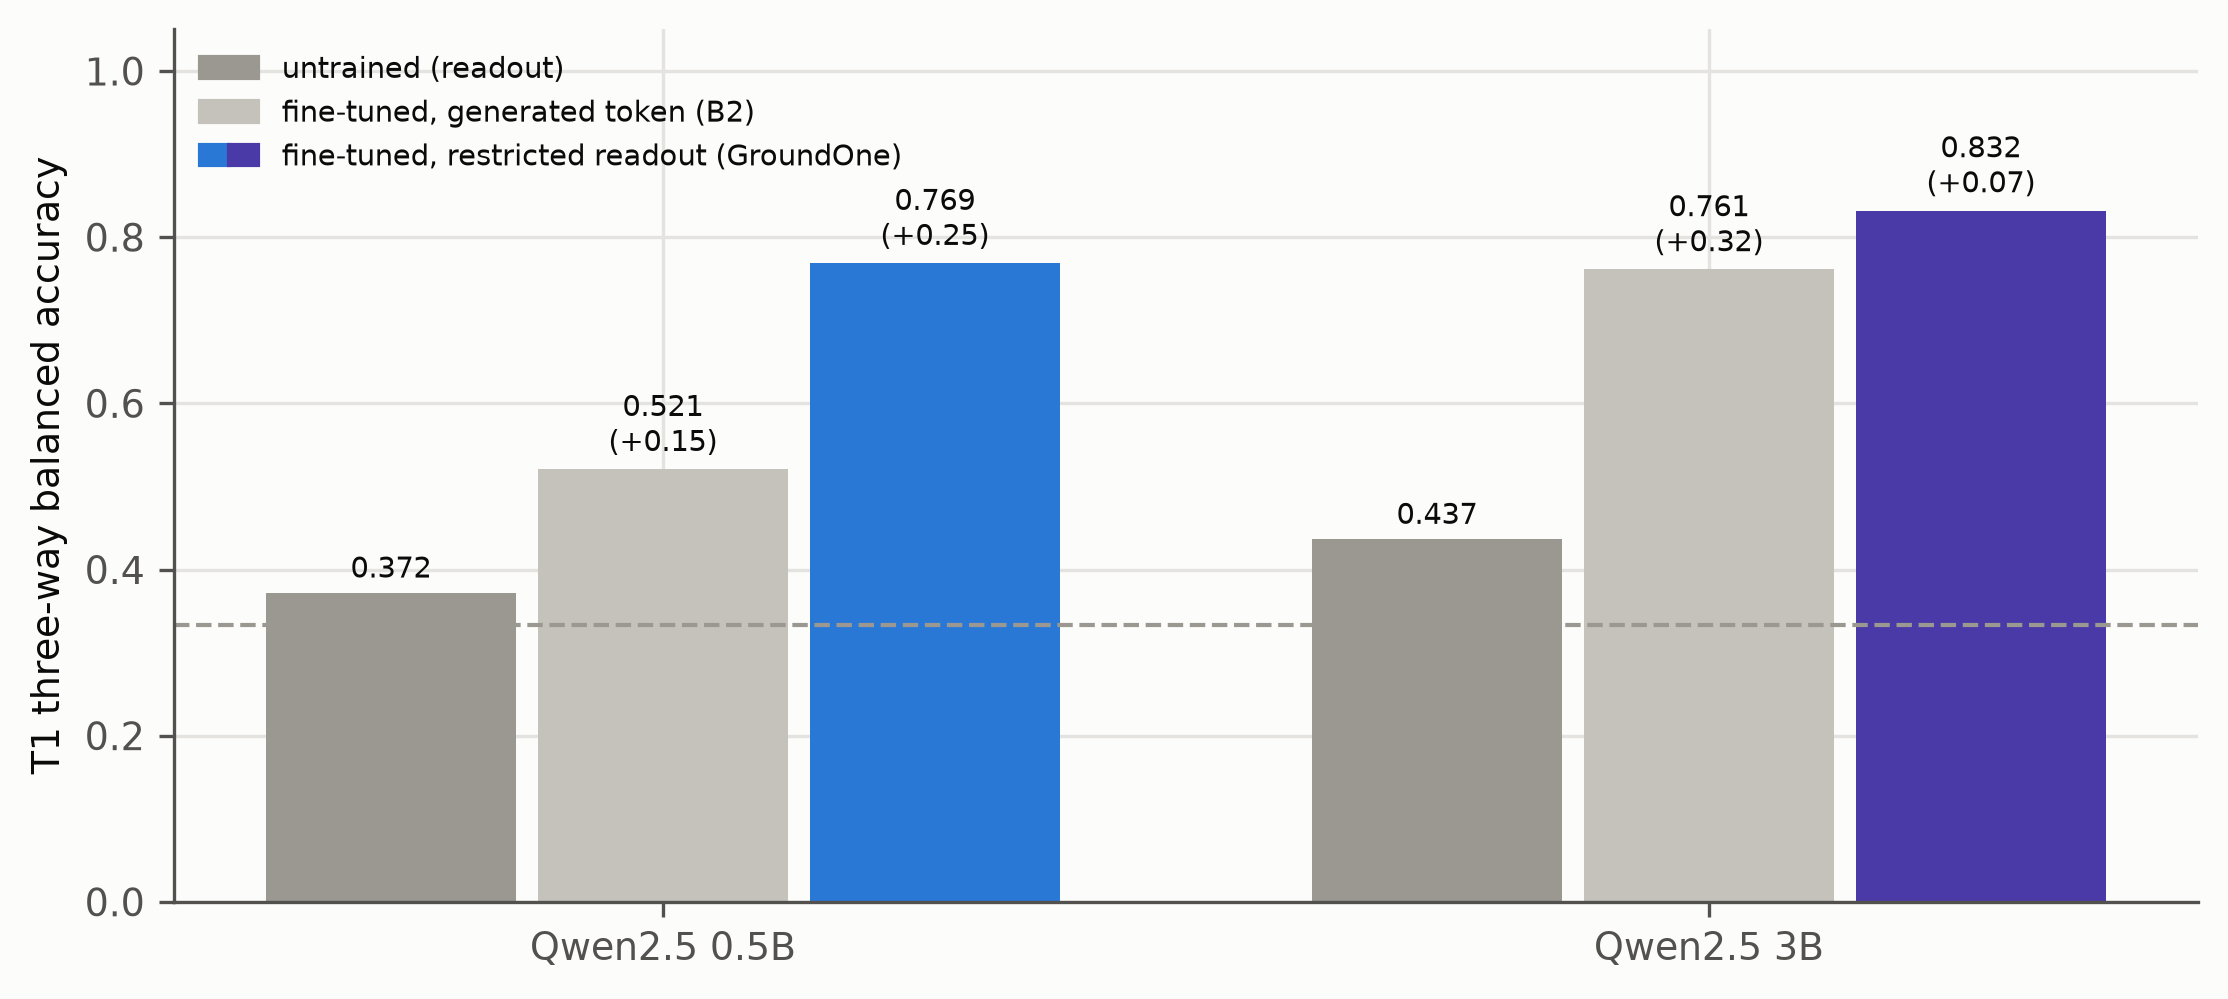
\includegraphics[width=\textwidth]{images/results/gain_decomposition.png}
\caption{Where the accuracy of GroundOne on T1 comes from: the same base model untrained (readout, design a), trained but
with the decision taken from the token it would generate (control B2, format failures counted as errors) and trained
with the restricted readout. The gain over the previous step is shown in brackets. The untrained 3B is evaluated on 600
answers; the dashed line marks the chance level.}
\label{fig:disc-gains}
\end{figure}

\paragraph{Calibration (RQ3).} A temperature and a bias fitted on the dev set align the probabilities with the
frequencies observed on the test set of the same domain, and the calibrated probabilities make selective prediction
effective. Two lessons hold beyond GroundOne. The first is that the Expected Calibration Error alone is not enough to
rank systems. After the same calibration, LLM judges whose probabilities barely separate the classes reach the same ECE as
GroundOne, and only the AUROC and the AURC reveal the difference. The second is that decisions and probabilities must be
derived consistently. If the most probable calibrated class is chosen, the decision collapses towards the majority
class; a threshold fitted on the dev set, instead, recovers the balanced decision and keeps the label consistent with the
probability shown to the user. As the results on VitaminC show, finally, calibration holds only for the distribution on
which it was fitted.

\paragraph{Cost on the device (RQ4).} The verifier fits comfortably in the 16\,GB laptop. During training the memory in
use peaks at 2.6\,GB with the 0.5B and at 5.9\,GB with the 3B. Verifying a long answer takes 0.41 seconds with the 0.5B
and 2.57 with the 3B, and the energy is on average 5.5 and 33 joules per answer. The 0.5B fits an interactive budget;
the 3B, instead, is slower than continuous interactive use would require, unless verification runs on request, as in
the application of Chapter~\ref{ch:studio}, and it trades time for accuracy. The energy measurements qualify the speed
results. A single long prefill draws more power than token-by-token decoding, so the energy saved is smaller than the
time saved, and the higher speed should not be read as an equal saving of battery. The verifier also coexists with a
generator in the same process: together with a 4-bit 3B generator, the peak memory is 6.1\,GB with the 3B and 3.3\,GB
with the 0.5B. The whole evaluation runs without any network access, with results identical bit for bit, and the 8-bit
weights cost no accuracy compared with bf16 ones (Section~\ref{sec:results-locality}). The retriever adds little: in the
application of Chapter~\ref{ch:studio}, with the generator, GroundOne 3B and the embedding model loaded together, the
memory allocated by MLX peaks at 6.2\,GB during one question and at 6.9\,GB after a session of twelve questions, with the KV cache of the sources already read.

The economic cost should also be read with care (Table~\ref{tab:disc-cost}). Verifying 10{,}000 answers with GroundOne
takes an amount of energy that, at the European average household electricity price~\cite{eurostat2026electricity}, is
worth less than one euro cent with the 0.5B and about three cents with the 3B. Entrusting the same verification to a
hosted LLM judge, at the providers' list prices~\cite{anthropic2026pricing,openai2026pricing,google2026geminipricing}, costs
instead from about one dollar with the cheapest models to more than two hundred with the top-tier ones. The ratio is
thus two to four orders of magnitude, but in absolute terms cheap LLM judges remain inexpensive, and the comparison takes into
account neither the purchase of the hardware nor the quality of hosted LLM judges, which this thesis did not measure. The
decisive argument for local verification therefore remains independence: the documents never leave the machine and the
service does not depend on an external provider.

\begin{table}[htbp]
\centering
\caption{Indicative cost of verifying 10{,}000 RAG answers. Hosted LLM judges: standard-tier list prices, accessed on 19
October 2026, with about 900 input tokens per answer (median T1 document and answer plus the instructions) and the
output tokens measured for the 3B LLM judges of this thesis (36 for the terse LLM judge, 248 for the verbose one). GroundOne:
measured net chip energy multiplied by the EU average household electricity price (0.29~€/kWh, second half of 2025).
Hardware cost and caching or batch discounts are excluded.}
\label{tab:disc-cost}
\small
\begin{tabular}{lccc}
\toprule
System & \makecell{Input / output price\\(USD per Mtoken)} & \makecell{Terse\\judge} & \makecell{Verbose\\judge} \\
\midrule
\makecell[l]{Claude Haiku 5.5,\\gpt-6-luna} & 0.10 / 0.50 & 1.1 USD & 2.2 USD \\
Gemini 3.5 Flash-Lite & 0.30 / 2.50 & 3.6 USD & 8.9 USD \\
Gemini 3.8 Flash & 0.75 / 3.75 & 8.2 USD & 16 USD \\
\makecell[l]{Claude Sonnet 5.5, gpt-6.1-sol,\\Gemini 4 Argon} & 2.00 / 10.00 & 22 USD & 43 USD \\
Claude Opus 5.5 & 4.00 / 20.00 & 43 USD & 86 USD \\
gpt-6-astra & 10.00 / 50.00 & 109 USD & 215 USD \\
\midrule
GroundOne 0.5B (local) & \multicolumn{3}{c}{0.015 kWh, about 0.004 €} \\
GroundOne 3B (local) & \multicolumn{3}{c}{0.092 kWh, about 0.03 €} \\
\bottomrule
\end{tabular}
\end{table}

\paragraph{Beyond a binary score (RQ5).} The three-way output separates contradicted from not-mentioned sentences well in
data-to-text, the task in which RAGTruth concentrates its contradictions. It separates them much less in question
answering and summarisation, where contradictions are rare in the training data. The 3B improves considerably on this
front, which suggests that what the small model lacks is more varied contradictions in training rather than a different
architecture. The strict and lenient policies and the threshold are all derived from the same three probabilities. The
user can therefore change the notion of error without retraining the model, which no binary verifier allows.
Figure~\ref{fig:disc-when} summarises these indications as a decision tree.

\begin{figure}[htbp]
\centering
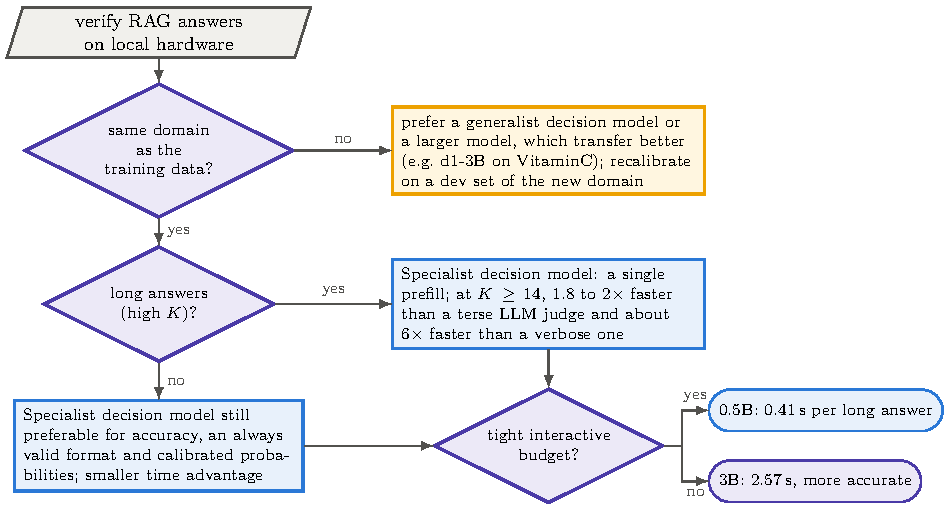
\includegraphics[width=\textwidth]{images/diagrams/disc_when_specialist_tikz.pdf}
\caption{When a specialist decision model pays off, according to the results of this thesis. The summary is qualitative:
the times refer to the M4 laptop and to answers with 14 or more sentences, and the out-of-domain transfer is the one
observed on LLM-AggreFact and VitaminC.}
\label{fig:disc-when}
\end{figure}

\section{Limitations}
\label{sec:disc-limitations}

\paragraph{One platform and one family of models.} Every result comes from a single laptop, a single runtime and a
single model family. Latency and energy depend on the hardware and on the implementation: what should hold elsewhere are
the ratios between methods, not the absolute values. The latency of GroundOne is compared neither with that of the
encoders nor with that of the general-purpose decision models, because these ran in different runtimes and under
conditions that would make the comparison unfair (see also the paragraph ``One machine'' in
Section~\ref{sec:disc-threats}).

\paragraph{Training stability.} Two completed runs of the 0.5B agree on all aggregate metrics, but a third run collapsed
in its early stages and was stopped. The training recipe has no gradient clipping and uses AdamW without bias correction,
two known causes of unstable fine-tuning~\cite{pascanu2013difficulty,mosbach2021stability}. Either could explain the
collapse, but neither hypothesis was tested. The 3B, moreover, was trained only once, on half of the training answers,
and its variability across seeds remains unknown.

\paragraph{Training data.} RAGTruth is the only training source. Its contradictions are concentrated in data-to-text and,
outside that task, are learned only in part. The models, moreover, rely partly on lexical overlap. When support is
expressed in different words, the sentence looks unsupported; when a sentence copies the source except for a small
change, the change often goes unnoticed. This blind spot shrinks as the model grows, but it remains the main limitation of
both.

\paragraph{Scope of the decision.} Verification is carried out sentence by sentence and only against the retrieved
document. A sentence that is true in the world but absent from the document therefore counts as not mentioned: this is
the right behaviour for groundedness, but not for fact checking. Sentences without checkable content are excluded by a
rule, and the segmentation itself can split or merge claims differently from a human reader. Finally, the verdict on a
sentence depends only on the document and on the sentences that precede it.

\paragraph{Language.} All training and test data are in English, so GroundOne was trained, calibrated and measured only on
English documents and answers. The base model Qwen2.5 is multilingual~\cite{qwen2024qwen25}, but it was not measured how
far the learned specialisation transfers to other languages, nor whether the calibration remains valid: the calibration
fitted on RAGTruth does not transfer even to another English domain such as VitaminC. Use with documents or answers in
another language, or in different languages from each other, therefore requires a new evaluation.

\paragraph{Contexts made of several documents.} When the answer is written from several retrieved passages, GroundOne
reads them concatenated as a single document, as in RAGTruth question answering. Three limits remain, however. The first
concerns length: in training, document and answer never exceed 2{,}048 tokens, so a longer context falls outside the
distribution on which the model was measured and must be split into chunks, keeping for each sentence the highest
support probability, as on LLM-AggreFact; a fact that requires combining two different chunks may then be missed. The
second concerns conflicting sources: when one passage supports a sentence and another contradicts it, the expected
verdict is not uniquely defined, and RAGTruth contains no such cases. The third concerns attribution: GroundOne states
whether a sentence is supported, but not by which passage; a first, unevaluated prototype is described in
Section~\ref{sec:studio-flow}.

\paragraph{Statistical scope.} The bootstrap intervals describe the variability of the test set, not that of training.
Moreover, about sixty comparisons were tested without correction for multiple testing. For this reason the conclusions
rest on effects far from zero, and differences on LLM-AggreFact and VitaminC smaller than the spread between seeds are
not claimed. Several baselines, finally, were evaluated on subsamples, which widens their intervals.

\section{Threats to validity}
\label{sec:disc-threats}

\paragraph{Labels.} The distinction between contradicted and not-mentioned sentences rests on the RAGTruth annotators,
whose agreement on the type of hallucination is not published. In addition, a recent re-annotation of the RAGTruth test
split found considerably more hallucinated answers than the original labels indicate~\cite{yu2026retromorphic}. The test
set may therefore under-count the minority classes. For this reason the three-way results on RAGTruth should always be
read together with those on VitaminC, whose labels have a measured inter-annotator agreement. LLM-AggreFact, finally,
unifies the labels of eleven datasets of different quality, and some of its columns are known to be noisy.

\paragraph{In-domain advantage.} GroundOne is trained on RAGTruth. Its results on the RAGTruth test set and on the
RAGTruth column of LLM-AggreFact therefore favour it with respect to systems trained elsewhere. Conversely, VitaminC is
part of the data from which the training of MiniCheck-RoBERTa descends. Each comparison is reported with the relevant
caveat, and the conclusions rest on the overall pattern across the three test sets rather than on a single one.

\paragraph{Baseline configuration.} LLM judges are sensitive to their prompts. Their prompts were fixed before
looking at the test results, and the prompt of the equal-output LLM judge was chosen on the dev set on the basis of format
validity only. Output parsing was lenient, to the LLM judges' advantage. Decoding was not constrained by a grammar, which
mostly affects the format failures of the smallest model. Neither an LLM judge fine-tuned on the same data nor a larger LLM judge
was evaluated: the comparison therefore measures what an LLM judge of the same size offers without training. Rizzo-Flow was
run with 4-bit weights, because the 8-bit model did not fit in memory beside the operating system, and this may
understate its accuracy. d1-3B, finally, was run zero-shot and, on LLM-AggreFact, only on a subsample. It received the
questions used for all decision-model baselines, which may not be the phrasing that suits it best.

\paragraph{Contamination.} The base models were pretrained on large web corpora that may include parts of the public
test sets\footnote{Data \emph{contamination} occurs when examples from a test set appear, even only in part, in the
pretraining data of a model. A contaminated model may remember the examples instead of judging them, and its scores on
that test set are then too optimistic.}. The same base models, however, used untrained as baselines, reach near-chance
accuracy on the three-way task. Contamination therefore cannot explain the gains due to training; for the absolute
values, instead, it cannot be ruled out entirely.

\paragraph{One machine.} All measurements of time and energy come from a single laptop, an Apple M4 with 16\,GB, and a
single runtime, MLX. The cost model of Chapter~\ref{sec:local} predicts that the advantage of a decision model holds on
every class of local hardware, because it rests on the difference between prefill and decoding, which vendors and
independent studies observe everywhere. The lower bounds on the cost of decoding computed in that chapter for other
machines also follow from published specifications. The actual speed-ups on a discrete graphics card, a DGX Spark or a
smartphone, however, were not measured. Their size depends on the balance between computation and bandwidth of each
machine: the cost model supports the direction of the advantage, not its magnitude.
